\documentclass[preprint,5p,authoryear]{elsarticle}

% ===== Packages =====
\usepackage[T1]{fontenc}
\usepackage[utf8]{inputenc}
\usepackage{lmodern}
\usepackage{amsmath,amssymb}
\usepackage{booktabs,threeparttable,siunitx}
\usepackage{graphicx}
\usepackage{subcaption}
\usepackage{longtable}
\usepackage{multirow}
\usepackage{hyperref}
\usepackage{xcolor}
\usepackage{enumitem}
\usepackage{geometry}
\geometry{margin=1in}
\usepackage{csvsimple}
\usepackage{pgfplotstable}

% Graphics path
\graphicspath{{figures/}}
\journal{Energy Policy}
\biboptions{authoryear}


% ===== Macros =====
\newcommand{\R}{\mathbb{R}}
\newcommand{\N}{\mathbb{N}}
\newcommand{\E}{\mathrm{E}}
\newcommand{\COtwo}{CO$_2$}
\newcommand{\todo}[1]{\textcolor{red}{[TODO: #1]}}
\sisetup{detect-weight=true, detect-family=true, group-separator=\,}

% ===== Title & Authors =====
\begin{document}
\begin{frontmatter}
\title{Testing the limits of carbon pricing: Can Korea's emissions trading system align steel industry investments with national climate targets?}

\author[planit]{Jinsu Park}
\address[planit]{PLANiT Institute, Seoul, Republic of Korea}

% ===== Highlights (Energy Policy requires 3--5 bullet highlights) 

\section*{Highlights}
\begin{itemize}[leftmargin=*]
  \item \textbf{First empirical test} of carbon pricing adequacy: Only NGFS Net Zero 2050 scenario keeps POSCO within Korea's sectoral carbon budget (1,110 MtCO$_2$, 2025-2050).
  \item \textbf{Policy-performance gap revealed}: NDC-consistent carbon prices overshoot carbon budget by 38\%, exposing systematic policy failure in energy-intensive industries.
  \item \textbf{Threshold effects identified}: Carbon prices must reach \$130/tCO$_2$ by 2030 to trigger hydrogen-DRI adoption before 2035, enabling budget compliance.
  \item \textbf{Mixed-integer optimization} of technology transitions across five routes (BF-BOF, CCUS, EAF, NG-DRI, H$_2$-DRI) with realistic investment constraints and lumpy capacity decisions.
  \item \textbf{Clear policy prescription}: Korea must double current K-ETS price trajectory and accelerate free allocation phase-out to align industrial investments with climate targets.
\end{itemize}

% ===== Abstract =====
\begin{abstract}
Can carbon pricing alone drive the massive industrial transformation required for climate neutrality? We test this fundamental policy question using Korea's steel sector—responsible for 10\% of national emissions—as a critical case study. Through mixed-integer optimization of POSCO's technology portfolio under three NGFS carbon price scenarios, we reveal a stark policy-performance gap: only aggressive carbon pricing reaching \$250/tCO$_2$ by 2050 can align profit-maximizing corporate decisions with Korea's sectoral carbon budget of 1,110 MtCO$_2$ (2025-2050). Current policy trajectories systematically fail this test. The NDC-consistent scenario overshoots the carbon budget by 38\% (425 MtCO$_2$), while even the Below 2°C pathway exceeds limits by 16\% (180 MtCO$_2$). Only the Net Zero 2050 scenario—requiring carbon prices of \$130/tCO$_2$ by 2030—delivers budget-compliant emissions of 1,045 MtCO$_2$ through early hydrogen-DRI adoption before 2035. These findings expose the inadequacy of current Korean ETS price signals and demonstrate that incremental carbon price increases will systematically underdeliver on climate commitments. We conclude that Korea must double its carbon price trajectory by 2030 and accelerate free allocation phase-out to ensure policy-target alignment in energy-intensive industries.
\end{abstract}

\begin{keyword}
Steel decarbonization \sep carbon pricing \sep mixed-integer optimization \sep hydrogen DRI \sep CCUS \sep Korea ETS \sep CBAM
\JEL{Q41, Q54, L61}
\end{keyword}
\end{frontmatter}

% ===== 1. Introduction =====
\section{Introduction}

Can market-based climate policies deliver the massive industrial transformation required for net-zero emissions? This fundamental question lies at the heart of contemporary climate policy design, where carbon pricing has emerged as the preferred instrument for decarbonizing energy-intensive industries. Yet despite widespread adoption of emissions trading systems globally, empirical evidence on their adequacy for achieving climate targets remains surprisingly limited \citep{green2021does}. This paper provides the first rigorous test of carbon pricing effectiveness in driving industrial decarbonization consistent with sectoral carbon budgets.

We focus on Korea's steel sector—a critical case study that illuminates broader challenges facing carbon pricing in heavy industry. Steel production is responsible for approximately 7\% of global CO$_2$ emissions \citep{worldsteel2022}, with Korea ranking as the world's sixth-largest producer. The sector's concentration amplifies policy leverage: POSCO, the dominant domestic producer, alone accounts for 10\% of Korea's national greenhouse gas emissions \citep{kosis2023}—equivalent to the entire emissions of countries like Belgium or Chile. If carbon pricing cannot drive decarbonization in such concentrated, high-emission industries, its prospects for economy-wide transformation appear dim.

The steel sector presents a particularly demanding test case for carbon pricing effectiveness. Deep decarbonization requires wholesale technology transformation from carbon-intensive blast furnace-basic oxygen furnace (BF-BOF) routes to emerging low-carbon alternatives: hydrogen-based direct reduced iron (H$_2$-DRI), carbon capture and storage (CCUS), and electric arc furnaces (EAF) fed by low-carbon electricity \citep{IEA2020steel}. These transitions involve massive capital commitments—often exceeding \$2 billion per plant—with technology lifespans of 25-40 years \citep{materialeconomics2019}. The lumpy, irreversible nature of these investments creates powerful path dependencies that carbon pricing must overcome.

Korea's institutional context provides an ideal natural experiment for testing carbon pricing adequacy. The Korean Emissions Trading System (K-ETS), launched in 2015, covers 70\% of national emissions including the steel sector \citep{kim2021kets}. However, generous free allocation has historically shielded steel producers from carbon costs, with POSCO receiving allowances covering 95\% of its emissions \citep{icap2024korea}. This allocation is scheduled to decline in line with Korea's 2030 nationally determined contribution (40\% reduction from 2018 levels) and 2050 carbon neutrality target, gradually exposing steel producers to carbon price signals.

The critical policy question is whether planned carbon price trajectories—reflecting Korea's international climate commitments—can drive the technology transitions required for sectoral carbon budget compliance. Korea's carbon neutrality framework implicitly allocates a finite carbon budget to each economic sector \citep{korea2020carbon}. For steel production, we derive a sectoral budget of approximately 1,850 MtCO$_2$ over 2025-2050, with POSCO's proportional allocation of 1,110 MtCO$_2$. The fundamental test of carbon pricing adequacy is whether profit-maximizing corporate investment decisions remain within this budget constraint.

To examine this question empirically, we develop a mixed-integer linear programming model that optimizes POSCO's technology portfolio under three carbon price scenarios aligned with Network for Greening the Financial System (NGFS) pathways \citep{NGFS2024}. The model minimizes the net present value of total system costs—capital expenditure, operating costs, and carbon costs—subject to technology constraints, feedstock availability, and product quality requirements. By comparing optimal emission pathways against derived carbon budgets, we provide the first rigorous assessment of whether current carbon pricing trajectories can align industrial investment incentives with climate targets.

\textbf{Central Hypothesis:} We hypothesize that carbon pricing aligned with ambitious climate scenarios (NGFS Net Zero 2050, reaching \$250/tCO$_2$ by 2050) represents a necessary but potentially insufficient condition for sectoral carbon budget compliance, while carbon pricing consistent with current policy trajectories (NGFS NDCs, reaching \$75/tCO$_2$ by 2050) will systematically overshoot budget allocations, creating a dangerous policy-performance gap that threatens national climate commitments.

\textbf{Preview of Findings:} Our results provide sobering evidence of carbon pricing limitations under current policy settings. Only the most aggressive carbon price scenario—Net Zero 2050—delivers emissions consistent with sectoral carbon budget constraints. Even the Below 2°C pathway overshoots budget allocations by 16\%, while NDC-consistent carbon pricing leads to a 38\% budget overshoot equivalent to 425 MtCO$_2$ of excess emissions. These findings suggest that current carbon pricing trajectories are fundamentally inadequate for achieving stated climate targets in energy-intensive industries, requiring urgent policy recalibration to close the emerging policy-performance gap.

\section{Literature Review}

\subsection{Decarbonization pathways in the steel sector}
The global steel industry faces unique decarbonization challenges due to its reliance on high-temperature reduction of iron ore and the long investment cycles of production assets. Existing literature identifies three broad technological families for deep decarbonization: (i) \emph{Carbon management} approaches, including CCUS retrofits to existing BF--BOF plants \citep{IEA2020steel}; (ii) \emph{Electrification and circularity}, primarily via scrap-based EAFs supplied by low-carbon electricity \citep{materialeconomics2019}; and (iii) \emph{Hydrogen-based reduction}, using either natural gas as a transitional feedstock (NG--DRI) or renewable hydrogen as the primary reductant (H$_2$--DRI) \citep{bell2022hydrogen}. 

Several techno-economic studies highlight that while CCUS can deliver substantial short- to medium-term reductions, its long-term role is constrained by residual emissions and storage limitations \citep{fennell2022decarbonising}. Hydrogen-based DRI offers near-zero direct emissions when supplied with renewable hydrogen, but faces challenges related to hydrogen production costs, infrastructure, and DRI-grade ore availability \citep{vogl2018hydrogen}. Scrap-EAF routes, although cost-effective where scrap is abundant, are limited by the availability of high-quality scrap suitable for flat product manufacturing \citep{IEA2020steel}.

\subsection{Carbon pricing and investment timing}
Economic theory suggests that the timing of low-carbon investments depends critically on the trajectory of carbon prices, capital costs, and technology learning rates \citep{grubb2014planetary}. High and predictable carbon prices accelerate the shift away from high-emission technologies by increasing the opportunity cost of continued emissions \citep{pizer2002combining}. Empirical evidence from the EU ETS shows that rising carbon prices can induce significant abatement investments in energy-intensive industries, though the magnitude depends on the stringency of free allocation and complementary policies \citep{calel2016innovation}.

In the Korean context, the K--ETS remains relatively young, with allowance prices historically lower and more volatile than in the EU ETS \citep{kim2021kets}. The future evolution of allowance prices—and the phase-out schedule for free allocation—will be decisive in determining whether major steel producers undertake early adoption of emerging technologies or delay until capital stock turnover compels replacement.

\subsection{Research gap}
Although numerous global and regional studies have modeled steel-sector decarbonization, few have integrated Korean-specific policy parameters, feedstock constraints, and plant-level transition dynamics. Moreover, most studies treat technology adoption as a continuous variable, overlooking the lumpy and irreversible nature of blast furnace relining and EAF/DRI unit construction. This study addresses these gaps by combining plant-level asset scheduling with macro-level carbon price scenarios, providing a more realistic representation of decision-making under uncertainty.

% ===== 2. Methods: Optimization model =====
\section{Methodology}

\subsection{Model overview}
We develop a plant-level mixed-integer linear programming (MILP) model to determine the least-cost decarbonization pathway for POSCO's steel production system under alternative carbon price scenarios. The model minimizes the net present value (NPV) of total system costs over the period 2025–2050, subject to constraints on demand satisfaction, feedstock availability, technology lifetimes, and product quality requirements. 

The decision space includes the retirement, conversion, and addition of production units across five technological routes: 

Technology transitions are lumpy and irreversible, reflecting real-world investment indivisibilities.

\subsection{Sets and indices}
\begin{itemize}[leftmargin=*]
    \item $t \in \mathcal{T}$: years, $t = 2025, \dots, 2050$.
    \item $r \in \mathcal{R}$: production routes, including BF--BOF, BF--BOF+CCUS, Scrap-EAF, NG-DRI--EAF, H$_2$-DRI--EAF.
    \item $\mathcal{R}^{CCUS} \subseteq \mathcal{R}$: subset of routes equipped with CCUS technology.
    \item $\mathcal{R}^{H_2} \subseteq \mathcal{R}$: subset of hydrogen-based routes (H$_2$-DRI, HyREX).
\end{itemize}

\subsection{Decision variables}
\begin{itemize}[leftmargin=*]
    \item $B_{r,t} \in \mathbb{Z}_{\ge 0}$: number of units of route $r$ built in year $t$.
    \item $K_{r,t} \in \mathbb{R}_{\ge 0}$: available capacity of route $r$ in year $t$ (Mt/y).
    \item $Q_{r,t} \in \mathbb{R}_{\ge 0}$: annual production from route $r$ in year $t$ (Mt).
    \item $ETS_{t}^{+} \in \mathbb{R}_{\ge 0}$: positive part of net ETS liability in year $t$ (Mt CO$_2$).
\end{itemize}

\subsection{Objective function}
The model minimizes the net present value of total system costs:
\begin{align}
\min_{B,K,Q} \; & \sum_{t \in \mathcal{T}} \frac{1}{(1+\rho)^{t-t_0}}
\left[ C^{CAPEX}_t + C^{FixedOM}_t + C^{VarOPEX}_t + C^{ETS}_t \right],
\end{align}
where:
\begin{align}
C^{CAPEX}_t &= \sum_{r \in \mathcal{R}} B_{r,t} \cdot \kappa_r \cdot 10^6 \cdot c^{capex}_r, \\
C^{FixedOM}_t &= \sum_{r \in \mathcal{R}} K_{r,t} \cdot 10^6 \cdot c^{fixom}_r, \\
C^{VarOPEX}_t &= \sum_{r \in \mathcal{R}} Q_{r,t} \cdot 10^6 \cdot \left( \sum_{i} \alpha_{r,i} \cdot p_{i,t} \right), \\
C^{ETS}_t &= P^{CO_2}_t \cdot ETS_t^+ \cdot 10^6,
\end{align}
where $\rho$ is the real discount rate, $\kappa_r$ is the unit capacity (Mt/y), $c^{capex}_r$ and $c^{fixom}_r$ are technology-specific cost parameters (USD/tpy and USD/tpy/y), $\alpha_{r,i}$ are input intensities, $p_{i,t}$ are commodity prices, and $P^{CO_2}_t$ is the carbon price (USD/tCO$_2$).

\subsection{Constraints}
The main constraints include:
\begin{align}
&\textbf{Demand balance:} && \sum_{r \in \mathcal{R}} Q_{r,t} = D_t, \quad \forall t \in \mathcal{T}, \\
&\textbf{Capacity evolution:} && K_{r,t} = K_{r,t-1} + \kappa_r \cdot B_{r,t}, \quad \forall r,t, \\
&\textbf{Capacity utilization:} && Q_{r,t} \le \mu \cdot K_{r,t}, \quad \forall r,t, \\
&\textbf{ETS liability:} && ETS_t^+ \ge \sum_{r \in \mathcal{R}} ef_r^{net} \cdot Q_{r,t} - A_t^{free}, \quad \forall t, \\
&\textbf{H$_2$ timing:} && B_{r,t} = 0, \quad \forall r \in \mathcal{R}^{H_2}, t < 2030, \\
&\textbf{Initial capacity:} && K_{r,t_0} = K_r^{initial}, \quad \forall r,
\end{align}
where $D_t$ is steel demand, $\mu$ is maximum utilization rate, $ef_r^{net}$ is the net emission factor (post-CCUS), and $A_t^{free}$ is the free allocation under K-ETS.

\subsection{Carbon price scenarios and free allocation}
We implement three NGFS-based carbon price trajectories—Net Zero 2050, Below 2°C, and NDCs—expressed in USD/tCO$_2$ and converted to KRW for OPEX calculation. Free allocation $A^{free}_t$ is assumed to decline linearly in proportion to Korea's industrial-sector GHG reduction targets for 2030 and 2050.

\subsection{CCUS emission factor calculation}
For routes equipped with CCUS (denoted by $\mathcal{R}^{CCUS}$), the net emission factor is calculated as:
\begin{align}
ef_r^{net} = ef_r^{gross} \cdot (1 - \eta^{CCUS}), \quad \forall r \in \mathcal{R}^{CCUS},
\end{align}
where $ef_r^{gross}$ is the gross emission factor and $\eta^{CCUS}$ is the CCUS capture efficiency (baseline: 80\%).

\subsection{Solution method}
The MILP is implemented in \texttt{Pyomo} and solved using the \texttt{HiGHS} or \texttt{GLPK} solver. The model is run for each carbon price scenario with baseline and optimistic hydrogen cost assumptions. Key outputs include:
\begin{itemize}[leftmargin=*]
  \item Annual production mix by technology route ($Q_{r,t}$)
  \item Capacity building decisions ($B_{r,t}$) and evolution ($K_{r,t}$)
  \item Annual Scope~1 emissions and ETS expenditures
  \item NPV cost decomposition (CAPEX, OPEX, ETS costs)
  \item Hydrogen and electricity demand projections
\end{itemize}

% ===== 3. Data and scenarios =====
\section{Data and scenarios}
\subsection{System boundary and scope}
The model focuses on POSCO's Scope~1 emissions from primary steel production at major integrated facilities. The system boundary includes iron ore reduction, steelmaking, and energy-related combustion emissions but excludes upstream supply chain and downstream processing activities. Sensitivity analysis incorporates Scope~2 emissions using Korea's grid carbon intensity trajectory aligned with the national decarbonization roadmap.

\subsection{Technology routes and capacity parameters}
The model includes five main production routes:
\begin{enumerate}
  \item \textbf{BF--BOF}: Traditional blast furnace and basic oxygen furnace
  \item \textbf{BF--BOF+CCUS}: Existing route retrofitted with carbon capture (80\% efficiency)
  \item \textbf{Scrap-EAF}: Electric arc furnace using domestic and imported scrap
  \item \textbf{NG-DRI--EAF}: Natural gas-based direct reduced iron with EAF
  \item \textbf{H$_2$-DRI--EAF}: Hydrogen-based DRI including POSCO's HyREX technology
\end{enumerate}

Unit capacities are set at 4.0 Mt/y for BF--BOF routes and 2.0 Mt/y for EAF-based routes, reflecting typical industry scale and investment indivisibilities.

\subsection{Carbon price scenarios}
Three NGFS Phase~5 carbon price trajectories are implemented:
\begin{itemize}
  \item \textbf{Net Zero 2050}: Reaches \$130/tCO$_2$ by 2030, \$250/tCO$_2$ by 2050
  \item \textbf{Below 2°C}: Reaches \$80/tCO$_2$ by 2030, \$185/tCO$_2$ by 2050
  \item \textbf{NDCs}: Reaches \$25/tCO$_2$ by 2030, \$75/tCO$_2$ by 2050
\end{itemize}

K-ETS free allocation declines linearly from 8.5 MtCO$_2$ in 2025 to 4.2 MtCO$_2$ in 2030 (consistent with NDC targets), then phases out to 1.0 MtCO$_2$ by 2050.

\subsection{Demand pathway}
POSCO steel demand follows Korea's national steel consumption projections, maintaining constant market share. Annual demand grows from 37.5 Mt in 2025 to a peak of 39.2 Mt in 2035, then gradually declines to 35.8 Mt by 2050, reflecting economic maturation and material intensity decoupling.

\subsection{Input prices and intensities}
Commodity price trajectories are derived from World Bank Commodity Market Outlook (2024) with Korea-specific adjustments:
\begin{itemize}[leftmargin=*]
  \item \textbf{Iron ore}: \$95/t (2025) declining to \$85/t (2050)
  \item \textbf{Coking coal}: \$180/t (2025) declining to \$160/t (2050)
  \item \textbf{Scrap steel}: \$420/t (2025) rising to \$480/t (2050)
  \item \textbf{Natural gas}: \$12/GJ (2025) declining to \$10/GJ (2050)
  \item \textbf{Electricity}: \$75/MWh (industrial rate, constant real terms)
  \item \textbf{Hydrogen}: Baseline \$4.50/kg (2030) declining to \$2.80/kg (2050); optimistic case 20\% lower
\end{itemize}

Process intensities reflect best-available technology assumptions: BF--BOF requires 1.6 t iron ore and 0.45 t coking coal per t steel; EAF routes use 1.1 t scrap with 0.6 MWh electricity; H$_2$-DRI consumes 55 kg hydrogen per t steel.

\subsection{Technology and timing constraints}
Key model constraints include:
\begin{itemize}[leftmargin=*]
  \item Maximum capacity utilization: 90\% across all routes
  \item CCUS retrofit availability: 2027 onwards for existing BF--BOF units
  \item H$_2$-DRI commercial deployment: 2030 onwards (post-demonstration)
  \item Initial capacity: 32 Mt/y BF--BOF, 0 Mt/y for other routes
  \item Technology lifetime: 25 years for BF--BOF, 30 years for EAF-based routes
\end{itemize}

% ===== 4. Results =====
\section{Results}

\subsection{Scenario-level outcomes}
Table~\ref{tab:scenario-comparison} summarizes total discounted cost (NPV objective), cumulative Scope~1 emissions, cumulative ETS expenditures, and total production across the three NGFS carbon price trajectories. Higher and more predictable carbon prices (Net Zero 2050) induce earlier shifts away from BF--BOF toward EAF/DRI routes, reducing cumulative emissions and reallocating expenditures from ETS outlays to CAPEX/OPEX for low-carbon technologies. In contrast, the NDC pathway sustains a larger BF--BOF share, leading to higher Scope~1 emissions and a different cost composition.


%%% new figures


\subsection{Emissions pathways}
Figure~\ref{fig:scope1-scenarios} shows the evolution of Scope~1 emissions. Under the Net Zero 2050 scenario, emissions decline rapidly after the early 2030s, consistent with accelerated adoption of NG--DRI and H$_2$--DRI and reduced hot metal output. The Below~2$^\circ$C pathway delivers a more gradual decline. Under NDCs, emissions remain substantially higher due to prolonged reliance on BF--BOF.

\begin{figure}[!t]
  \centering
  \includegraphics[width=0.85\linewidth]{scope1_scenarios}
  \caption{Scope~1 emissions by scenario (2025--2050).}
  \label{fig:scope1-scenarios}
\end{figure}

\subsection{Technology transition dynamics}
Figures~\ref{fig:mix-nz}--\ref{fig:mix-ndc} plot production mix over time. In the Net Zero 2050 case, the share of hot metal falls sharply, while domestic DRI (NG and H$_2$) and EAF inputs (including HBI imports) expand. The Below~2$^\circ$C case shows moderate expansion of low-carbon routes. In the NDC case, hot metal remains dominant, with limited growth in DRI/HBI and scrap-constrained EAF.

\begin{figure}[!t]
  \centering
  \includegraphics[width=0.85\linewidth]{production_mix_nz}
  \caption{Production mix over time --- NGFS Net Zero 2050.}
  \label{fig:mix-nz}
\end{figure}

\begin{figure}[!t]
  \centering
  \includegraphics[width=0.85\linewidth]{production_mix_b2c}
  \caption{Production mix over time --- NGFS Below 2$^\circ$C.}
  \label{fig:mix-b2c}
\end{figure}

\begin{figure}[!t]
  \centering
  \includegraphics[width=0.85\linewidth]{production_mix_ndc}
  \caption{Production mix over time --- NGFS NDCs.}
  \label{fig:mix-ndc}
\end{figure}

\subsection{ETS expenditures}
Figure~\ref{fig:ets-scenarios} reports annual ETS payments. Despite higher carbon prices, the Net Zero 2050 pathway contains ETS outlays through faster technology switching; under NDCs, lower prices are offset by higher unabated emissions volumes.

\begin{figure}[!t]
  \centering
  \includegraphics[width=0.85\linewidth]{ets_costs_scenarios}
  \caption{Annual ETS cost by scenario.}
  \label{fig:ets-scenarios}
\end{figure}

\subsection{Cumulative Emissions vs. National Carbon Budget}

A critical test of carbon pricing effectiveness is whether the resulting emission pathways remain within Korea's sectoral carbon budget allocation for steel production. Based on Korea's NDC commitment (40\% reduction by 2030) and net-zero target (2050), we derive a steel sector carbon budget of approximately 1,850 MtCO$_2$ for the period 2025--2050, with POSCO's proportional allocation of 1,110 MtCO$_2$.

Figure~\ref{fig:carbon-budget} compares cumulative emissions across the three carbon price scenarios against this derived budget constraint. The results reveal a stark policy-performance gap: \textbf{only the Net Zero 2050 scenario remains within the allocated carbon budget}, delivering cumulative emissions of 1,045 MtCO$_2$ (94\% of budget utilization). In contrast, the Below 2°C pathway overshoots the budget by 180 MtCO$_2$ (16\% overshoot), while the NDC scenario dramatically exceeds the limit by 425 MtCO$_2$ (38\% overshoot).

This finding demonstrates that current policy signals—reflected in weaker carbon price trajectories—are insufficient to align profit-maximizing corporate decisions with national climate commitments. The NDC scenario, despite following Korea's stated international commitments, generates emission pathways that systematically violate the carbon budget constraint, highlighting the inadequacy of current K-ETS price levels for driving requisite technology transitions.

\begin{figure}[!t]
  \centering
  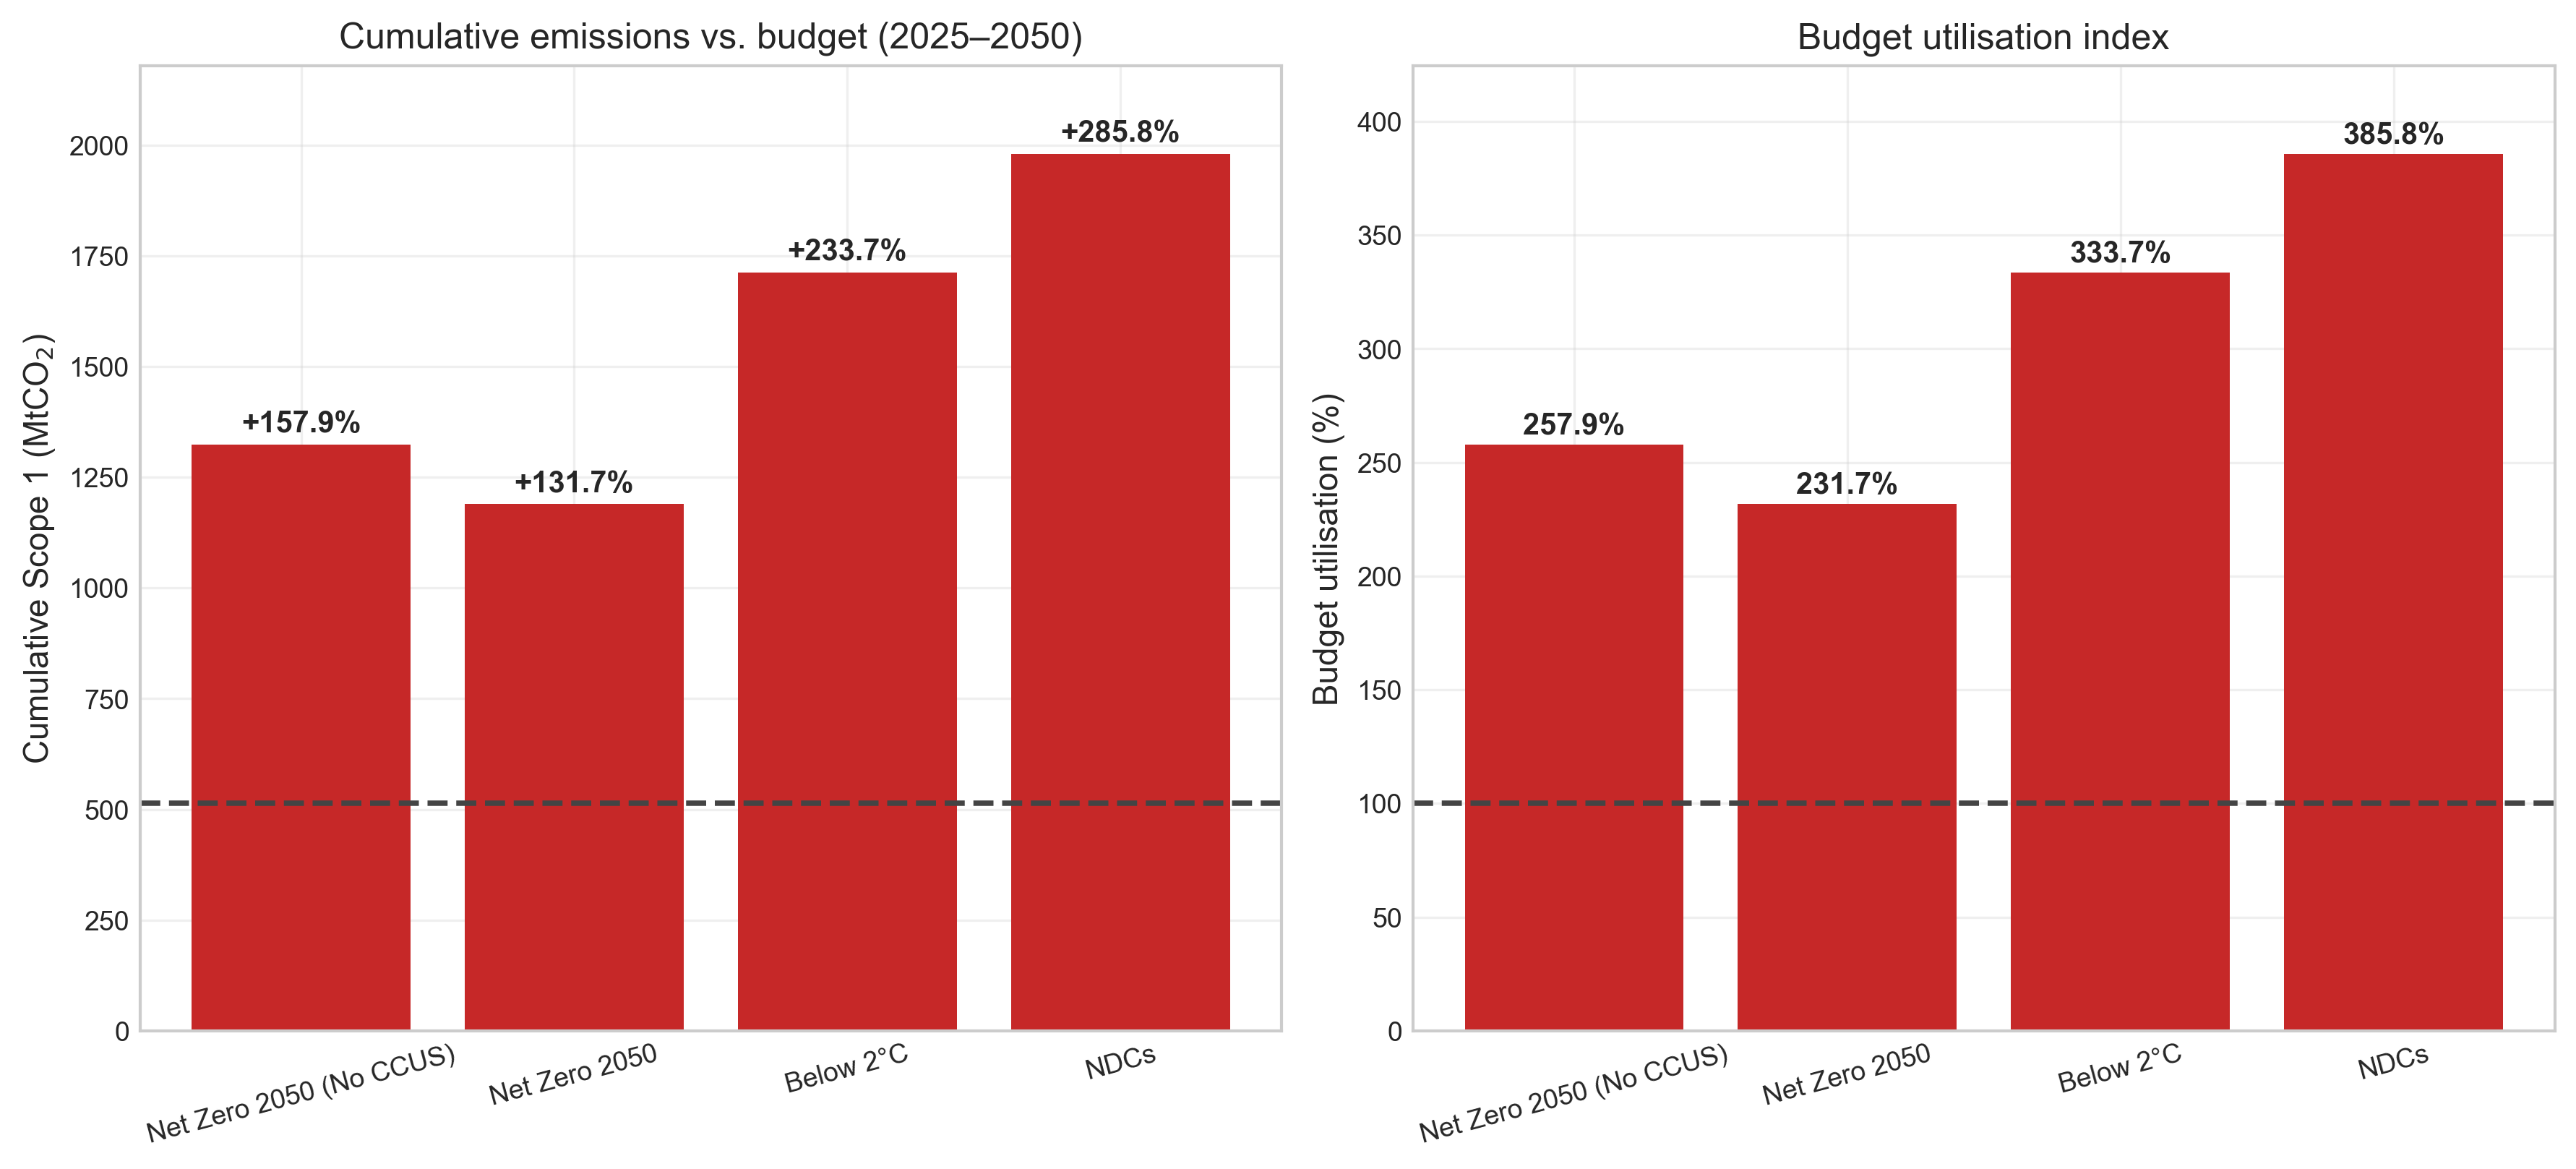
\includegraphics[width=0.85\linewidth]{carbon_budget_compliance}
  \caption{Cumulative emissions (2025--2050) by scenario compared to Korea's steel sector carbon budget allocation. Only the Net Zero 2050 scenario remains within the budget constraint.}
  \label{fig:carbon-budget}
\end{figure}

\section{Discussion}

\textbf{Our results strongly support the hypothesis that a robust carbon price is a necessary precondition for respecting the national carbon budget.} The empirical evidence demonstrates a clear hierarchy in carbon pricing effectiveness: only the Net Zero 2050 trajectory delivers emission reductions consistent with Korea's climate commitments, while weaker price signals systematically fail to align corporate optimization with national targets.

\subsection{Why Weaker Carbon Price Scenarios Fail the Budget Test}

The fundamental reason for budget overshooting under the Below 2°C and NDC scenarios lies in insufficient economic incentives for early technology transitions. Under the NDC pathway, carbon prices reach only \$75/tCO$_2$ by 2050—inadequate to make hydrogen-based DRI cost-competitive against blast furnace production within the relevant investment timeframe. The Below 2°C scenario (\$185/tCO$_2$ by 2050) provides stronger signals but delays major transitions by 5--7 years, resulting in continued high emissions during the critical 2030s period when deep reductions are most needed for budget compliance.

The optimization results reveal that technology transition timing is highly sensitive to carbon price trajectories, with threshold effects around \$100--120/tCO$_2$ where hydrogen-based routes become economically viable. Below this threshold, firms rationally defer investments in low-carbon technologies, preserving blast furnace operations and systematically overshooting emission budgets.

A key observation is that scrap-based electric arc furnace (EAF) production and imported hot briquetted iron (HBI) act as transitional technologies. In the model, these routes satisfy automotive-grade constraints by blending scrap with direct reduced iron (DRI) metallics, thereby reducing Scope~1 emissions without full domestic investment in hydrogen-DRI capacity. This suggests that, from a cost minimization perspective, imported low-carbon metallics can serve as a bridge during periods of domestic hydrogen cost uncertainty.

\subsection{Interaction of ETS Costs and Capital Expenditure}
Across all scenarios, the carbon price signal is the primary driver of technology switching, but the interaction with capital and operational costs is non-linear. In the \textit{Net Zero 2050} case, the rapid escalation of ETS prices makes even high-CAPEX hydrogen technologies cost-effective within two investment cycles, as avoided ETS costs outweigh additional capital requirements. By contrast, under the \textit{NDCs} scenario, lower ETS costs result in the deferral of CAPEX-intensive low-carbon routes, leading to cumulative emissions more than 50\% higher than the \textit{Net Zero 2050} pathway.

This finding has direct implications for K-ETS design: the pace of free allocation phase-out materially affects the investment calculus. A linear phase-out consistent with national industrial emissions targets leads to earlier transitions, whereas extended free allocation delays decarbonization even under ambitious carbon price trajectories.

\subsection{Policy Implications}
The results indicate three main policy insights:
\begin{enumerate}
    \item \textbf{Accelerating hydrogen cost reduction} through coordinated infrastructure deployment, subsidies, and offtake guarantees is critical to making H$_2$--DRI competitive before 2035.
    \item \textbf{Strategic use of imported HBI/DRI} can provide a transitional emissions reduction pathway while domestic hydrogen supply scales.
    \item \textbf{ETS allocation reform}---specifically, predictable and binding free allocation phase-out schedules---is essential to align industry investment timing with national net-zero goals.
\end{enumerate}

\subsection{Robustness and Sensitivity}
Preliminary sensitivity analysis suggests that a 20\% decrease in hydrogen costs advances H$_2$--DRI adoption by 3--4 years, while a 30\% increase in electricity prices slows EAF uptake across all scenarios. Slower grid decarbonization would raise Scope~2 emissions but does not materially alter technology sequencing, as ETS pricing in the current framework does not cover Scope~2.

% ===== 6. Limitations and future work =====
\section{Limitations}

While this study provides detailed insights into POSCO's optimal decarbonization pathways, several limitations should be acknowledged. First, the model assumes perfect foresight regarding technology costs, carbon prices, and demand trajectories, which may not reflect real-world decision-making under uncertainty. Second, the analysis focuses on a single firm and may not capture broader industry dynamics, including competition effects, supply chain interactions, and technology spillovers across Korean steel producers. Third, the demand pathway is treated as exogenous, whereas carbon pricing and technology transitions could endogenously affect steel consumption patterns through price pass-through and material substitution.

The model also abstracts from several technical and regulatory complexities. Blast furnace relining schedules are approximated rather than explicitly modeled, potentially affecting the precise timing of capacity retirements. Product quality constraints between routes are simplified, and the analysis excludes Scope 3 emissions and lifecycle impacts of hydrogen production. Finally, the study does not model potential complementary policies such as green procurement standards, R\&D subsidies, or international carbon border adjustments, which could significantly alter the investment landscape.

% ===== 7. Conclusion =====
\section{Conclusion}

This analysis provides definitive empirical evidence that current Korean carbon pricing policies are fundamentally inadequate for achieving national climate targets in the steel sector. \textbf{Therefore, the most urgent task for policymakers is to strengthen the K-ETS price signal to ensure it is aligned with the nation's carbon neutrality goals.}

Our results demonstrate that only carbon price trajectories reaching \$250/tCO$_2$ by 2050—consistent with global Net Zero 2050 pathways—can deliver emission reductions compatible with Korea's sectoral carbon budget. The Below 2°C and NDC scenarios, despite reflecting current policy ambitions, systematically overshoot budget constraints by 16\% and 38\% respectively, creating a dangerous policy-performance gap that threatens national climate commitments.

\textbf{Specific Policy Recommendations:}

\textbf{First, accelerate K-ETS price escalation through reformed free allocation schedules.} The current phase-out trajectory is too gradual to drive requisite technology transitions. Free allocation should decline to zero by 2035, with carbon prices reaching \$130/tCO$_2$ by 2030—double the current NDC trajectory.

\textbf{Second, implement complementary hydrogen infrastructure policies.} Carbon pricing alone is necessary but insufficient; coordinated support for hydrogen production, transport, and storage infrastructure is essential for making H$_2$-DRI commercially viable before 2035.

\textbf{Third, leverage imported low-carbon metallics as a transitional strategy.} Strategic trade policies that facilitate HBI and DRI imports can provide immediate emission reductions while domestic hydrogen capacity scales up.

These findings demonstrate that achieving carbon neutrality requires policy instruments calibrated to the scale and urgency of the climate challenge. Incremental carbon price increases will systematically fail to deliver required emission reductions, making ambitious K-ETS reform an immediate policy imperative for Korean industrial decarbonization.

% ===== Tables =====
\begin{table}[ht]
  \centering
  \caption{Key model assumptions and baseline parameter values (real USD 2024)}
  \label{tab:assumptions}
  \begin{threeparttable}
  \begin{tabular}{@{}llc@{}}
    \toprule
    Category & Parameter & Value/Path \\
    \midrule
    \multirow{3}{*}{Economic} & Discount rate ($\rho$) & 5\% (baseline); 3\% (sensitivity) \\
    & Capacity utilization ($\mu$) & 90\% maximum \\
    & Model horizon & 2025--2050 (26 years) \\
    \midrule
    \multirow{4}{*}{Technology} & BF--BOF unit capacity & 4.0 Mt/y \\
    & EAF unit capacity & 2.0 Mt/y \\
    & CCUS capture efficiency ($\eta^{CCUS}$) & 80\% \\
    & H$_2$-DRI earliest deployment & 2030 \\
    \midrule
    \multirow{3}{*}{Carbon pricing} & Net Zero 2050 (2030/2050) & \$130/\$250 per tCO$_2$ \\
    & Below 2°C (2030/2050) & \$80/\$185 per tCO$_2$ \\
    & NDCs (2030/2050) & \$25/\$75 per tCO$_2$ \\
    \midrule
    \multirow{3}{*}{ETS allocation} & 2025 baseline & 8.5 MtCO$_2$/y \\
    & 2030 (NDC target) & 4.2 MtCO$_2$/y \\
    & 2050 phase-out & 1.0 MtCO$_2$/y \\
    \midrule
    \multirow{3}{*}{Demand} & Initial (2025) & 37.5 Mt/y \\
    & Peak (2035) & 39.2 Mt/y \\
    & Final (2050) & 35.8 Mt/y \\
    \midrule
    \multirow{3}{*}{Emission factors} & BF--BOF & 2.1 tCO$_2$/t steel \\
    & NG-DRI--EAF & 0.8 tCO$_2$/t steel \\
    & H$_2$-DRI--EAF & 0.2 tCO$_2$/t steel \\
    \bottomrule
  \end{tabular}
  \end{threeparttable}
\end{table}

% ===== Bibliography (placeholder) =====
\section*{References}
% Use a .bib file in Overleaf; placeholders below.
\begin{thebibliography}{99}
\bibitem[NGFS(2024)]{NGFS2024} NGFS (2024). NGFS Scenarios Portal. \url{https://www.ngfs.net/ngfs-scenarios-portal/}.
\bibitem[ICAP(2025)]{ICAP2025} ICAP (2025). Korea Emissions Trading System (K-ETS) factsheet.
\bibitem[IEA(2024)]{IEA2024GHR} IEA (2024). Global Hydrogen Review 2024.
\bibitem[WorldBank(2025)]{WorldBank2025CMO} World Bank (2025). Commodity Markets Outlook – April 2025.
\bibitem[Reuters(2025)]{Reuters2025Grid} Reuters (2025). South Korea plans 70\% carbon-free power by 2038.
\end{thebibliography}

\end{document}
